\documentclass[10pt, twoside]{article}
\title{Why a combination, $\Combination{n}{k}$, is always a natural number? Different way to look at the answer accentuates the generation process of factors and prime numbers contained within a particular range of $1$ to $n$.}
\author{Amit Kumar}
\date{}
\usepackage[a4paper, margin=0.75in]{geometry}
\usepackage[page]{appendix}
\usepackage{amsmath}
\usepackage{amssymb}
\usepackage{mathtools}
\usepackage{xcolor}
\usepackage{ulem}
\usepackage{cancel}
\usepackage{listings}
\usepackage{pythonhighlight}
\usepackage{graphicx}
\usepackage{float}
\usepackage{url}
\usepackage{subfiles}
\usepackage{xr}
\newcommand*{\Permutation}[2]{{}^{#1}P_{#2}}%
\newcommand*{\Combination}[2]{\binom{#1}{#2}}%
\newcommand\bypassurl[1]{\textbf{URL:} \textit{#1}}
\newcommand{\floordivision}[2]{\left\lfloor \frac{#1}{#2} \right\rfloor}
\externaldocument{Appendices}
\begin{document}
	\maketitle
	\section{Abstract}
	 The concept of combination is crucial to layout groundwork for many fundamental sciences, finance and technical domains. There are multiple known methods to show that the combination (binomial coefficient) is integral in nature. This article approaches the same concept with simple non-inductive algebraic steps that can be followed by a wide range of audiences. This article separates an $\Combination{n}{k}$ into mutually exclusive and collectively exhaustive cases and then shows for each case that any term in a denominator have at least one corresponding multiple in the numerator. All $k$ for a particular $n$ (for an $\Combination{n}{k}$) are visualized through plots to gain better understanding. In the context of the plots, this different way of looking at a Combination $\Combination{n}{k}$, gives hindsights into the generation process of factors and prime numbers contained within a particular range of $1$ to $n$.
	\section{Introduction}
	From countless ages, it has been desired to know the number of ways an arrangement can be obtained or selected out of many possible ways.
	
	Permutations and Combinations have become fundamental concepts with wide ranging applications in almost every sphere of academic studies or technical endeavors. While a permutation, $\Permutation{n}{k}$, tells how many number of ways $k$ objects can be arranged out of $n$ objects, if we are interested in \textit{exact order of the choosen $k$ items} \cite{PrincTechCombinatorics}.
		\begin{equation}
			\Permutation{n}{k} = \frac{n!}{(n-k)!}  \; \text{where n,k} \in \mathbb{N}  \; \text{and} \; 1 \leq k \leq n
		\end{equation}
		 \textit{e.g.} Number of possibilities to choose $5$ items out of $9$ choices, we will write as $\Permutation{9}{5} =\frac{9!}{(9-5)!}$ (see a nice introduction \cite{ProbabilityKIndle}).
		 It is easy to show that $n!$ (in the numerator) can be broken into a multiplication constituting two parts: one going from $n$ to $(n-k+1)$ and other going from $(n-k)$ to $1$. The denominator can also be written as multiplication of numbers from {\color{blue}$(n-k)$} to {\color{blue}$1$} as below.
		 \begin{align}
		 	\Permutation{n}{k} &= \frac{n!}{(n-k)!} \nonumber \\
		 	&= \frac{(n)\times(n-1)\cdots\times(n-k+1)\times\color{blue}(n-k)\times(n-k-1)\cdots\times3\times2\times1}{\color{blue}(n-k)\times(n-k-1)\times(n-k-2)\cdots\times3\times2\times1} \nonumber \\
		 	&= (n)\times(n-1)\cdots\times(n-k+1) \label{CondensedEquationPermutation}
		 \end{align}
	 	It is evident that the terms in \textbf{\color{blue}blue fonts} will cancel each other, in the numerator and the denominator, and we will be left with a product of integer sequence going from $n$ to $(n-k+1)$. Since each participating number in the product is a natural number, the net product is also a natural number.
	 	
	 	Combination, $\Combination{n}{k}$ represents number of ways $k$ elements out of $n$ can be choosen, \textit{without any regard to order between the choosen items} \cite{PrincTechCombinatorics}. Below are equivalent representations of a combination.
	\begin{align}
	\Combination{n}{k} &= {}^nC_k = C(n, k)  \\
					   &= \frac{\color{blue}\Permutation{n}{k}}{k!} \label{ConnectionBetweenPermutationAndCOmbination}\\	
					   &= \frac{\color{blue}n!}{{\color{blue}(n-k)!}\times(k)!} \label{FractionalDefinitionOfCombination}
	\end{align} 
	where n! means factorial of n and is defined as $n\times(n-1)\times(n-2)\cdots3\times2\times1$. 
		The results (value of combinations) have been observed to be integers (empirically, over and over again based on calculations) for a particular choice of n and k. The focus of this paper is a proof that holds, irrespective of any choice of n and k, and one that transcends manual calculations everytime to show the integral nature. This paper aims to demonstrate non-inductively and algebraically that for each denominator term there is at least one term in the numerator that is a multiple of it. Thus all the terms in the denominator will be cancelled and the final value of a combination will `always collapse to an integer (more correctly a natural number)'. At the end of it we visualize our results through graphs and we find an interesting but also a simple connection with the generation process of factors and prime numbers contained within the range $1$ to $n$. We conclude this article by showing that prime numbers do not arise randomly but they have a simple and systematic generation algorithm. To show effectiveness of this algorithm we start with a \textbf{single prime number, 2,} and generate the first 1000 prime numbers. These \textbf{generated} 1000 primes match exactly the first 1000 \textbf{known} prime numbers.
	\section{Proofs}
 	\subsection{Why Combination $\Combination{n}{k}$ is a natural number?}
 	Combination is the number of arrangements, when the order \textit{does not} matter and is given by \cite{PrincTechCombinatorics}:\newline
 	\begin{equation}
 		\Combination{n}{k} = \frac{n!}{(n-k)!\times(k)!} \; \text{where n,k} \in \mathbb{N} \; \text{and} \; 1 \leq k \leq n
 	\end{equation}
 	This time we can cancel the denominator's k!
 	\begin{align*}
 		\Combination{n}{k} &= \frac{(n)\times(n-1)\cdots\times(k+1)\times\color{blue}(k)\times(k-1)\cdots\times3\times2\times1}{(n-k)\times(n-k-1)\cdots\times3\times2\times1\times\color{blue}(k)\times(k-1)\cdots\times3\times2\times1}\\
 		&= \frac{(n)\times(n-1)\cdots\times(k+1)}{(n-k)\times(n-k-1)\cdots\times3\times2\times1}
 	\end{align*}
 Thus it can be written down as the below (after cancelling common terms shown in \textbf{\color{blue}blue fonts}):
 \begin{equation}
 	\Combination{n}{k} = \frac{(n)\times(n-1)\cdots\times(k+2)\times(k+1)}{(n-k)\times(n-k-1)\cdots\times3\times2\times1} \label{reducedCombinationForm}
 \end{equation}
\subsubsection{Different possible values of $n$ and $k$ w.r.t each other.}
 If $\floordivision{n}{2}$ is defined as integer portion of division of $n$ by $2$, then we can see that one of the two statements, below, must be true:
 \begin{align}
 	n &= (\floordivision{n}{2} \times 2) \; \text{where $n$ is an even number} \label{nIsEven}\\
 	n &= (\floordivision{n}{2} \times 2) + 1 \; \text{where $n$ is an odd number} \label{nIsOdd}
 \end{align}
On a similar note, $k$ can be defined as six and six only possibilities w.r.t $n$:
\begin{align}
	k &= \floordivision{n}{2} \; \text{where $n$ is an \textbf{even number} }\label{kEqualsCase1}\\
	k &= \floordivision{n}{2} - l \; \text{where $n$ is an even number and } l \in \mathbb{N} , 1 \leq l \leq \floordivision{n}{2} \label{kEqualsCase2}\\
	k &= \floordivision{n}{2} + m \; \text{where $n$ is an even number and } m \in \mathbb{N} , 1 \leq m \leq \floordivision{n}{2} \label{kEqualsCase3}\\
	\cline{1-2}
	k &= \floordivision{n}{2} \; \text{where $n$ is an \textbf{odd number} }\label{kEqualsCase4}\\
	k &= \floordivision{n}{2} - l \; \text{where $n$ is an odd number and } l \in \mathbb{N} , 1 \leq l \leq (n-1)/2 \label{kEqualsCase5}\\
	k &= \floordivision{n}{2} + m \; \text{where $n$ is an odd number and } m \in \mathbb{N} , 1 \leq m \leq (n+1)/2) \label{kEqualsCase6}		
\end{align}
Let us take a few concrete examples to understand the equations from equation \eqref{nIsEven} to equation \eqref{kEqualsCase6}.\newline\newline
$\Combination{10}{0}$ means $n$ is even, $k = 0$ and $l=\floordivision{n}{2}=5$: Thus equations \eqref{nIsEven} and \eqref{kEqualsCase2} are realized.\newline\newline
$\Combination{10}{2}$ means n is even, $k = 2$ and $l=3$: Thus equations \eqref{nIsEven} and \eqref{kEqualsCase2} are realized.\newline\newline
$\Combination{10}{4}$ means $n$ is even, $k = 4$ and $l=1$: Thus equations \eqref{nIsEven} and \eqref{kEqualsCase2} are realized.\newline\newline
$\Combination{10}{5}$ means $n$ is even and $k = \floordivision{n}{2} = 5$: Thus equations \eqref{nIsEven} and \eqref{kEqualsCase1} are realized.\newline\newline
$\Combination{10}{6}$ means $n$ is even, $k = 6$ and $m=1$: Thus equations \eqref{nIsEven} and \eqref{kEqualsCase3} are realized.\newline\newline
$\Combination{10}{8}$ means $n$ is even, $k = 8$ and $m=3$: Thus equations \eqref{nIsEven} and \eqref{kEqualsCase3} are realized.\newline\newline
$\Combination{10}{10}$ means $n$ is even, $k = 10$ and $m= \floordivision{n}{2}=5$: Thus equations \eqref{nIsEven} and \eqref{kEqualsCase3} are realized.\newline\newline
$\Combination{11}{0}$ means $n$ is odd, $k = 0$ and $l=(n-1)/2=5$: Thus equations \eqref{nIsOdd} and \eqref{kEqualsCase5} are realized.\newline\newline
$\Combination{11}{2}$ means n is odd, $k = 2$ and $l=3$: Thus equations \eqref{nIsOdd} and \eqref{kEqualsCase5} are realized.\newline\newline
$\Combination{11}{4}$ means $n$ is odd, $k = 4$ and $l=1$: Thus equations \eqref{nIsOdd} and \eqref{kEqualsCase5} are realized.\newline\newline
$\Combination{11}{5}$ means $n$ is odd and $k = \floordivision{n}{2} = 5$: Thus equations \eqref{nIsOdd} and \eqref{kEqualsCase4} are realized.\newline\newline
$\Combination{11}{6}$ means $n$ is odd, $k = 6$ and $m=1$: Thus equations \eqref{nIsOdd} and \eqref{kEqualsCase6} are realized.\newline\newline
$\Combination{11}{8}$ means $n$ is odd, $k = 8$ and $m=3$: Thus equations \eqref{nIsOdd} and \eqref{kEqualsCase6} are realized.\newline\newline
$\Combination{11}{11}$ means $n$ is odd, $k = 11$ and $m= (n+1)/2=6$: Thus equations \eqref{nIsOdd} and \eqref{kEqualsCase6} are realized.\newline\newline
We can clearly see based on equations \eqref{kEqualsCase1} to \eqref{kEqualsCase6} that there are six possibilities that we separately need to take care and prove. In the following subsections, \ref{ProofkEqualsCase1} to \ref{ProofkEqualsCase6}, we will prove each of the above condition.
\subsubsection{Setting up the problem}\label{settingUpTheProblem}
Looking at the equation \eqref{reducedCombinationForm} it is clear that each term in the denominator can be written as $(n-k-x)$, where $x \in \mathbb{W}, 0 \leq x \leq (n-k-1)$ and each term in the numerator can be written as $(k+y)$, where $y \in \mathbb{N}, 1 \leq y \leq (n-k)$. Formalizing the two equations as below:
\begin{align}
	\text{denominator} &= \prod_{0}^{n-k-1}(n-k-x), \text{where $n$ and $k$ are constants and $x$ is the variable} \label{denominator}\\
	\text{numerator} &= \prod_{1}^{n-k}(k+y), \text{where $k$ is a constant and $y$ is the variable} \label{numerator}
\end{align}
Now we have to show that for every $(n-k-x)$, there exists a natual number \textbf{$a$} such that $a \times (n-k-x) = (k+y)$ holds true. i.e.
\begin{equation}
	a \times (n-k-x) = (k+y), \text{where $a \in \mathbb{N}$}  \label{MultipleOfAisAnswer}
\end{equation}
\subsubsection{$\Combination{n}{k}$ is always a natural number when equation \eqref{nIsEven} and \eqref{kEqualsCase1} hold true}\label{ProofkEqualsCase1}
\begin{align}
	a \times (n-k-x) &= (k+y) \nonumber \\
	a \times (2\times \floordivision{n}{2} - \floordivision{n}{2} -x) &= (\floordivision{n}{2}+y) \nonumber \\
	a \times(\floordivision{n}{2} -x) &= (\floordivision{n}{2} + y) \nonumber \\
	a &= \frac{(\floordivision{n}{2}+y)}{(\floordivision{n}{2}-x)} \nonumber\\
	y &= a\times(\floordivision{n}{2}-x) - \floordivision{n}{2} \nonumber \\
	y &= (a-1)\times \floordivision{n}{2} - a\times x \label{yEqualsCase1}
\end{align}
Let us take a couple of examples. \newline
For $\Combination{10}{5} \text{ and } x = 1$ we get the solution as below
\begin{align*}
	y &= (a-1)\times 5 - a \\
	y &= a \times (5 - 1) - 5 \\
	y &= a \times 4 - 5 \\
\end{align*}
Clearly if $a = 2$ we get a valid solution and we obtain $y=3$. Let us see what this means. This means that for denominator $(n-k-x) = (10-5-1) = 4$, we will get a corresponding numerator which will have its factor as $(k+y) = (5+3) = 8$. This is consistent. Let us take another example.\newline
For $\Combination{10}{5} \text{ and } x = 3$ we get the solution as below
\begin{align*}
	y &= (a-1)\times 5 - a \times 3 \\
	y &= a \times (5 - 3) - 5 \\
	y &= a \times 2 - 5 \\
\end{align*}
Clearly if $a = 3$ we get a valid solution and then $y=1$. This result can be interpreted as before. This means that for the denominator $(n-k-x) = (10-5-3) = 2$, we will get a corresponding numerator which will have its factor as $(k+y) = (5+1) = 6$. This is also consistent.\newline
For \eqref{yEqualsCase1}, we know that $x \in \mathbb{W}, 0 \leq x \leq (n-k-1)$ and $y \in \mathbb{N}, 1 \leq y \leq (n-k)$. These two conditions get simplified due to \eqref{kEqualsCase1} as $0 \leq x \leq (\floordivision{n}{2}-1)$. Let us put extreme conditions of $x$ to see if we can obtain a valid \textbf{$a$} for the denominator for every $y$.
\begin{align*}
	y &= (a-1)\times \floordivision{n}{2} - a\times 0 \text{ this is due to \eqref{yEqualsCase1}} \\
	y &= (a-1)\times \floordivision{n}{2}
\end{align*}
Clearly an a can be choosen such that R.H.S is a natural number. Similarly we can say that,
\begin{align*}
	y &= (a-1)\times \floordivision{n}{2} - a\times (\floordivision{n}{2}-1) \text{ this is due to \eqref{yEqualsCase1}} \\
	y &= \cancel{a\times \floordivision{n}{2}} - \floordivision{n}{2} -\cancel{a\times \floordivision{n}{2}} +a \\	
	y &= a - \floordivision{n}{2}
\end{align*}
Clearly an \textbf{$a$} can be choosen such that R.H.S is a natural number. Thus we saw that an $a$ is available in the range of extreme $x$ values and thus we always have an \textbf{$a$} so that every denominator is a factor for some numerator.$\blacksquare$
\subsubsection{$\Combination{n}{k}$ is always a natural number when equation \eqref{nIsEven} and \eqref{kEqualsCase2} hold true}\label{ProofkEqualsCase2}
\begin{align}
	a \times (n-k-x) &= (k+y) \nonumber \\
	a \times (2\times \floordivision{n}{2} - \floordivision{n}{2} + l - x) &= (\floordivision{n}{2} - l + y) \nonumber \\
	a &= \frac{(\floordivision{n}{2} - l + y)}{(\floordivision{n}{2} + l - x)} \nonumber \\
	y &= (a-1)\times \floordivision{n}{2} + l \times (a+1) - a\times x \label{yEqualsCase2}	
\end{align}
How do we interpret this? Let us see an example. \newline
$\Combination{10}{4}$. Here $n = 10$ and thus $\floordivision{n}{2} = 5, k = 4, l = \floordivision{n}{2} - k = 5 -4 = 1$. Furthermore let us assume that $x = 1$, i.e. the denominator is $(n-k-1)$ for which the factor containing numerator has to be found.\newline
Putting the above values in \eqref{yEqualsCase2}, we get
$y = (a-1)5+1(a+1)-a\times 1 = (a-1)5+1$\newline
Clearly $a = 2$ will solve the equation which is consistent with restrictions on $y$ and the value of $y$ will be $y=(2-1)\times5 + 1=6$. That means the corresponding multiples will reside in the numerator $(k+y)=(k+6)$.\newline
Putting all the values in equation \eqref{MultipleOfAisAnswer} should get us no contradiction.
\begin{align}
	a \times (n-k-x) &= (k+y) \nonumber \\
	2 \times (10-4-1) &= (4+6) \nonumber \\
	2 \times (5) &= (10) \nonumber \\
	10 &= 10 \nonumber
\end{align}
Please note that $a = 1$ will also give a consistent solution as $y=(1-1)\times5 + 1=1$, which means $(k+1)$ is the desired numerator. Please note that $(n-k-x)=(10-4-1)=5$ will have two numerators where the multiples reside, one in $(k+1)=5$ and other in $(k+6)=10$.
We will have an addditional example as $\Combination{10}{4}$ and $x = 3$. i.e. the denominator is $(n-k-3)$ and the corresponding numerator, $(k+y)$, has to be found. Using \eqref{yEqualsCase2}, we get $y = (a-1)5+1(a+1)-a*3 = (a-1)5+6$\newline. Again $a=3$ will solve the equation and $y$ will be $y=(3-1)\times5 +1+ 3*3=2$. That means the corresponding factor will reside in the numerator $(k+y)=(k+2)$.\newline. To see if it is consistent, we will have to put the values in \eqref{MultipleOfAisAnswer} and we will find that the equality holds.
\begin{align}
	a \times (n-k-x) &= (k+y) \nonumber \\
	2 \times (10-4-3) &= (4+2) \nonumber \\
	2 \times (3) &= (6) \nonumber \\
	6 &= 6 \nonumber
\end{align}
Now according to \eqref{denominator}, 
\begin{align}
	0 \leq x \leq (n-k-1) &= 0 \leq x \leq (2\times \floordivision{n}{2}-\floordivision{n}{2}+l-1) \nonumber \\
	&= 0 \leq x \leq (\floordivision{n}{2}+l-1) \label{LimitOfXforYEqualsCase2}
\end{align}
We will show that the equations are consistent at the extremes of $x$ and therefore must be true for other values of $x$ in between.\newline
Choosing $x=0$ in the equation \eqref{yEqualsCase2}, we get
\begin{align*}
	y &= (a-1)\times \floordivision{n}{2} + l \times (a+1) - a\times x \\
	y &= (a-1)\times \floordivision{n}{2} + l \times (a+1) - a\times 0 \\
	y &= (a-1)\times \floordivision{n}{2} + l \times (a+1)
\end{align*}
Since $l$ is $a \in \mathbb{N}$, so the minimum value $l$ can have is $1$. Thus the second term in the R.H.S. above will be positive. To make $y$ as positive integer, there is always a value of $a$ we can choose to satisfy this restriction.\newline
At the other extreme, choosing $x=(\floordivision{n}{2}+l-1)$, we get the below.
\begin{align*}
	y &= (a-1)\times \floordivision{n}{2} + l \times (a+1) - a\times (\floordivision{n}{2}+l-1) \\
	y &= a\times \floordivision{n}{2} - \floordivision{n}{2} +l\times a +l -a\times \floordivision{n}{2}-a\times\ l + a \\
	y &= \cancel{a\times \floordivision{n}{2}} - \floordivision{n}{2} +\cancel{l\times a} +l -\cancel{a\times \floordivision{n}{2}}-\cancel{a\times\ l} + a \\
	y &= a - \floordivision{n}{2} + l 
\end{align*}
Again it is evident that an $a$ can be choosen such that $y$ can be in a form consistent with assumptions. Thus we have shown that the equation \eqref{yEqualsCase2} is consistent and solvable at extremes of $x$ and thus must be solvable between. $\blacksquare$
\subsubsection{$\Combination{n}{k}$ is always a natural number when equation \eqref{nIsEven} and \eqref{kEqualsCase3} hold true}\label{ProofkEqualsCase3}
\begin{align}
	a \times (n-k-x) &= (k+y) \nonumber \\
	a \times (2\times \floordivision{n}{2} - \floordivision{n}{2} - m - x) &= (\floordivision{n}{2} + m + y) \nonumber \\
	a &= \frac{(\floordivision{n}{2} +m + y)}{(\floordivision{n}{2} -m - x)} \nonumber \\
	y &= (a-1)\times \floordivision{n}{2} - m \times (a+1) - a\times x \label{yEqualsCase3}	
\end{align}
Interpreting this result is as before through an example.\newline
$\Combination{10}{6}$. Here $n = 10$ and thus $\floordivision{n}{2} = 5, k = 6, m = k - \floordivision{n}{2} = 6 - 5 = 1$. Furthermore let us assume that $x = 1$, i.e. the denominator is $(n-k-1)$ for which the factor containing numerator has to be found.\newline.
Substituting the above values in \eqref{yEqualsCase3}, we get  $y = (a-1)5-m(a+1)-a*1 = (a-1)5-1(1+a)-a = (a-1)5-2a-1$\newline. 
It is easy to see that the equation is solved for $a = 3$. In such a case $y$ will be equal to $(3-1)*5-2*3-1 = 3$. i.e. for $(n-k-1)$, there is a multiple in $(k+3)$, where $n=10$ and $k=6$. It is trivial to verify this.
\begin{align*}
	a \times (n-k-x) &= (k+y) \\
	3 \times (10-6-1) &= (6+3) \\
	3 \times (3) &= (9) \\
	9 &= 9 
\end{align*}
As per \eqref{denominator}, 
\begin{align}
	0 \leq x \leq (n-k-1) &= 0 \leq x \leq (2\times \floordivision{n}{2}-\floordivision{n}{2}-m-1) \nonumber \\
	&= 0 \leq x \leq (\floordivision{n}{2}-m-1) \label{LimitOfXforYEqualsCase3}
\end{align}
We need to show that there is no contradiction at the extremes \eqref{yEqualsCase3} and thus it will hold true for middle values as well.
Choosing $x = 0$ in equation \eqref{yEqualsCase3} we arrive at,
\begin{align*}
	y &= (a-1)\times \floordivision{n}{2} - m \times (a+1) - a\times x \\
	y &= (a-1)\times \floordivision{n}{2} - m \times (a+1) - a\times 0 \\
	y &= (a-1)\times \floordivision{n}{2} - m \times (a+1)
\end{align*}
 The above should hold for $y \geq 1$. Thus
 \begin{align*}
 	(a-1)\times \floordivision{n}{2} \geq 1 +  m \times (a+1) \\
 	a\times \floordivision{n}{2} -m\times a \geq (1+m+\floordivision{n}{2}) \\
 	a \geq \frac{(1+m+\floordivision{n}{2})}{(\floordivision{n}{2}-m)}
 \end{align*}
The last equation is defined as long as $\floordivision{n}{2} \ge m$. This constraint is already in place due to the premise of \eqref{kEqualsCase3}. Thus a value of \textbf{$a$} can be computed such that \eqref{yEqualsCase3} is satisfied.\newline
Working at the other extreme of $x = (\floordivision{n}{2} - m -1)$ we observe the below.
\begin{align*}
	y &= (a-1)\times \floordivision{n}{2} -m \times(1+a) -a \times (\floordivision{n}{2} -m -1) \\
	y &= a\times \floordivision{n}{2} - \floordivision{n}{2} -m -m\times a -a \times \floordivision{n}{2} - a\times m + a \\
	y &= \cancel{a\times \floordivision{n}{2}} - \floordivision{n}{2} -m -\cancel{m\times a} -\cancel{a \times \floordivision{n}{2}} - \cancel{a\times m} + a \\
	y &= (a - \floordivision{n}{2}) - m
\end{align*}
As seen, $y$ has allowed solutions at both extremes as there is always an a that can be choosen to satisfy the constraints.$\blacksquare$
\subsubsection{$\Combination{n}{k}$ is always a natural number when equation \eqref{nIsOdd} and \eqref{kEqualsCase4} hold true}\label{ProofkEqualsCase4}
\begin{align}
	a \times (n-k-x) &= (k+y) \nonumber \\
	a \times (2\times \floordivision{n}{2} + 1 - \floordivision{n}{2} - x) &= (\floordivision{n}{2} + y) \nonumber \\
	a &= \frac{(\floordivision{n}{2} + y)}{(\floordivision{n}{2} + 1 - x)} \nonumber \\
	y &= (a-1)\times \floordivision{n}{2} + a - a\times x \label{yEqualsCase4}	
\end{align}
The best way to understand the above equation, as before, is through an example.\newline
In $\Combination{11}{5}$, $n=11$, $\floordivision{n}{2}=5=k$. Let $x$ be equal to $1$, then substituting the values in the above equation, we get,
\begin{align*}
	y = (a-1)\times 5 + a - a\times 1 \\
	y = (a-1)\times 5 + \cancel{a} - \cancel{a\times 1} \\
	y = (a-1)\times 5
\end{align*}
Clearly $a = 2$ will give a solution and $y$ will be equal to $5$. That means for the above setup for $(n-k-1)$, there will be a factor in $(k+5)$. It is easy to verify this.\newline
\begin{align*}
	a \times (n-k-x) &= (k+y) \nonumber \\
	2 \times (11-5-1) &= (5+5) \nonumber \\
	2 \times (5) &= (10) \nonumber \\
	10 &= 10
\end{align*}
Just like before we can appreciate that the equation \eqref{yEqualsCase4} has boundaries for extreme values of $x$. Thus if we show the lower extreme and upper extreme values of $x$ to have a consistent solution, then the proof must hold for values in between.\newline
We remember that $0 \leq x \leq (n-k-1)=0 \leq x \leq (2\times \floordivision{n}{2} + 1-\floordivision{n}{2}-1)=0 \leq x \leq \floordivision{n}{2}$. First we will check for the lower limit of $0$. Putting $0$ in equation \eqref{yEqualsCase4}, we get,
\begin{align*}
	y &= (a-1)\times \floordivision{n}{2} + a - a\times x \\
	y &= (a-1)\times \floordivision{n}{2} + a - a\times 0 \\
	y &= (a-1)\times \floordivision{n}{2} + a \\
\end{align*}
Clearly a value of $a$ can be choosen such that R.H.S satisfies the constraint that $y \in \mathbb{N}$. When we think of the other extreme, we obtain the following.
\begin{align*}
	y &= (a-1)\times \floordivision{n}{2} + a - a\times x \\
	y &= (a-1)\times \floordivision{n}{2} + a - a\times (n-k-1) \\
	y &= (a-1)\times \floordivision{n}{2} + a - a\times (2\times \floordivision{n}{2} + 1-\floordivision{n}{2}-1) \\
	y &= (a-1)\times \floordivision{n}{2} + a - a\times (\floordivision{n}{2}) \\
	y &= a - \floordivision{n}{2}
\end{align*}
Here also it is clear that a value of \textbf{$a$} can be choosen such that the R.H.S is greater than or equal to $1$. \newline
Thus we have shown that a valid $y$ can be obtained by choosing an appropriate $a$, for two extreme values of $x$.$\blacksquare$
\subsubsection{$\Combination{n}{k}$ is always a natural number when equation \eqref{nIsOdd} and \eqref{kEqualsCase5} hold true}\label{ProofkEqualsCase5}
\begin{align}
	a \times (n-k-x) &= (k+y) \nonumber \\
	a \times (2\times \floordivision{n}{2} + 1 - \floordivision{n}{2} +l - x) &= (\floordivision{n}{2} -l + y) \nonumber \\
	a &= \frac{(\floordivision{n}{2} -l + y)}{(\floordivision{n}{2} + 1 +l - x)} \nonumber \\
	y &= (a-1)\times \floordivision{n}{2} + l\times(a+1) - a\times x + a \label{yEqualsCase5}	
\end{align}
Let us find the value for an example. Suppose we are given $\Combination{11}{4}$. Here $n=11$, $\floordivision{n}{2}=5$, $k=4$, $l=1$ and let's say $x=1$. Then putting these values in the above equation, we get:
\begin{align*}
	y &= (a-1)\times \floordivision{n}{2} + l\times(a+1) - a\times x + a \\
	y &= (a-1)\times 5 + 1\times(a+1) - a\times 1 + a \\
	y &= (a-1)\times 5 + \cancel{1\times a}+ 1 - \cancel{a\times 1} + a \\
	y &= (a-1)\times 5 + 1 + a \\
\end{align*}
Clearly $a=1$ gives a solution and thus $y=2$. This argues that for $(n-k-1)$, there is a factor in $(k+2)$ for this example. i.e. for $(11-4-1)$ we have a factor in $(4+2)$. It is evident that $6$ is on both sides of the equation.\newline
Now we have to show that given an $x$ and $l$ and $n$, we can get a $y$ such that $y \in \mathbb{N}$. We will show for two extreme values of $x$, it should hold true for values in between.\newline
Let's recall that $0 \leq x \leq (n-k-1) = 0 \leq x \leq (2\times \floordivision{n}{2}+1-\floordivision{n}{2}+l-1) = 0 \leq x \leq (\floordivision{n}{2} + l)$. Starting with $x=0$ and substituting $x=0$ in equation \eqref{yEqualsCase5}.
\begin{align*}
	y &= (a-1)\times \floordivision{n}{2} + l\times(a+1) - a\times x + a \\
	y &= (a-1)\times \floordivision{n}{2} + l\times(a+1) - a\times 0 + a \\	
	y &= (a-1)\times \floordivision{n}{2} + l\times(a+1) + a \\		
\end{align*}
In the above each term on the right hand side is a positive integer and therefore the net value of $y$ is also going to be a positive integer and thus the restriction that $1 \leq y, y \in \mathbb{N}$\newline
Putting the other extreme value of $x$ in equation \eqref{yEqualsCase5}
\begin{align*}
	y &= (a-1)\times \floordivision{n}{2} + l\times(a+1) - a\times x + a \\
	y &= (a-1)\times \floordivision{n}{2} + l\times(a+1) - a\times (\floordivision{n}{2}+l) + a \\	
	y &= a\times \floordivision{n}{2} - \floordivision{n}{2} - l\times a + l -a\times \floordivision{n}{2} - a \times l + a \\
	y &= \cancel{a\times \floordivision{n}{2}} - \floordivision{n}{2} - \cancel{l\times a} + l -\cancel{a\times \floordivision{n}{2}} - \cancel{a \times l} + a \\
	y &= a - \floordivision{n}{2} + l \\
\end{align*}
Given the limits on $l$ as per equation \eqref{kEqualsCase5}, a value of $l$ can be found such that a consistent value of $y$ can be obtained. $\blacksquare$\\
\subsubsection{$\Combination{n}{k}$ is always a natural number when equation \eqref{nIsOdd} and \eqref{kEqualsCase6} hold true}\label{ProofkEqualsCase6}
\begin{align}
	a \times (n-k-x) &= (k+y) \nonumber \\
	a \times (2\times \floordivision{n}{2} + 1 - \floordivision{n}{2} -m - x) &= (\floordivision{n}{2} +m + y) \nonumber \\
	a &= \frac{(\floordivision{n}{2} +m  + y)}{(\floordivision{n}{2} + 1 +-m - x)} \nonumber \\
	y &= (a-1)\times \floordivision{n}{2} -m\times(a+1) - a\times x + a \label{yEqualsCase6}	
\end{align}
Let us see the equation \eqref{yEqualsCase6} in action. \newline
Suppose it is given that we have to work on $\Combination{11}{6}$, then $n=11,\floordivision{n}{2}=5,k=6,m=1$. Furthermore suppose $x=3$, i.e. we have to find the multiple of $(n-k-3)$ in the numerator.
\begin{align*}
	y &= (a-1)\times \floordivision{n}{2} -m\times(a+1) - a\times x + a \\
	y &= (a-1)\times 5 - 1\times(a+1) - a\times 3 + a \\
	y &= (a-1)\times 5 -1 -3\times a \\
	y &= 5\times a - 5 -1 -3\times a \\
	y &= 2\times a - 6
\end{align*}
Clearly there is a solution for $a = 4$. Once we have obtained, a then we can plug it in equation \eqref{yEqualsCase6} to obtain the value of $y$. We get,
\begin{align*}
	y &= (a-1)\times \floordivision{n}{2} -m\times(a+1) - a\times x + a \\
	y &= (4-1)\times 5 -1\times(4+1) - 4\times 3 + 4 \\
	y &= 15 - 5 -12 + 4 \\
	y &= 2
\end{align*}
Thus for $\Combination{11}{6}$, for the numerator $(n-k-3)$, there is a factor in $(k+2)$. It is easy to verify this using \eqref{MultipleOfAisAnswer}. Putting the values:
\begin{align*}
	4\times(11-6-3) &= (6+2)\\
	4\times 2 &= 8
\end{align*}
Thus we arrive at a consistent solution.\newline
What is left to be shown is that given an $x$, $m$ and $n$, we can always get a $y$ such that $y \in \mathbb{N}$. Since $x$ has limits in equation \eqref{yEqualsCase6}, it suffices to show that a consistent $y$ can be obtained always if consistent $y$ can be obtained at the lower and upper extremes.\newline
Now $0 \leq x \leq (n-k-1) = 0 \leq x \leq (2\times \floordivision{n}{2}+1-\floordivision{n}{2}-m-1) = 0 \leq x \leq (\floordivision{n}{2} -m)$. Given this premise, we first substitute the lower limit of $x$ which is $0$.
\begin{align*}
	y &= (a-1)\times \floordivision{n}{2} -m\times(a+1) - a\times x + a \\
	y &= (a-1)\times \floordivision{n}{2} -m\times(a+1) - a\times 0 + a \\
	y &= (a-1)\times \floordivision{n}{2} -m\times(a+1) + a \\
	y &= a\times(\floordivision{n}{2}-m+1) - (\floordivision{n}{2}+m) \\
\end{align*}
So as long as $a\times(\floordivision{n}{2}-m+1) - (\floordivision{n}{2}+m) \geq 1$, the RHS will be a natural number and consistent $y$ can be obtained.
\begin{align}
	a\times(\floordivision{n}{2}-m+1) - (\floordivision{n}{2}+m) &\geq 1 \nonumber \\
	a\times(\floordivision{n}{2}-m+1) &\geq (\floordivision{n}{2}+m+1) \nonumber \\
	a &\geq \frac{(\floordivision{n}{2}+m+1)}{(\floordivision{n}{2}-m+1)} \label{tempAforYequals6-1}
\end{align}
Thus for the above to hold true $(1+\floordivision{n}{2}-m) \geq 0$.\newline
Due to constraints imposed by \eqref{ProofkEqualsCase6} 
\begin{align*}
	m \leq (n+1)/2 \\
	m \leq (2\times \floordivision{n}{2} + 1 +1)/2 \\
	m \leq (2\times \floordivision{n}{2} + 2)/2 \\
	m \leq (\floordivision{n}{2}+1) \\
	0 \leq (1+\floordivision{n}{2}-m)
\end{align*}
So the requirement is already satisfied for \eqref{tempAforYequals6-1} and thus for $x=0$ it is always possible to have a $y \in \mathbb{N}$. Now let us see the other extreme of $x$ which is $(\floordivision{n}{2}-m)$. Putting this value in equation \eqref{yEqualsCase6}.
\begin{align*}
	y &= (a-1)\times \floordivision{n}{2} -m\times(a+1) - a\times x + a \\
	y &= (a-1)\times \floordivision{n}{2} -m\times(a+1) - a\times(\floordivision{n}{2}-m) + a\\
	y &= a\times \floordivision{n}{2} -\floordivision{n}{2} -m\times a - m -a\times \floordivision{n}{2} +a\times m + a \\
	y &= \cancel{a\times \floordivision{n}{2}} -\floordivision{n}{2} -\cancel{m\times a} - m -\cancel{a\times \floordivision{n}{2}} +\cancel{a\times m} + a \\
	y &= (a - \floordivision{n}{2}) -m 
\end{align*}
If $(a - \floordivision{n}{2}) -m \geq 1$, the RHS will always be a positive integer and a consistent $y$ can be obtained.
\begin{align}
	(a - \floordivision{n}{2}) -m  &\geq 1 \nonumber \\
	a &\geq (\floordivision{n}{2}+m+1) \label{tempAforYequals6-2}
\end{align}
Since the R.H.S is a positive integer it is always possible to get such a value of $a$ and thus $y$ can be obtained for the other extreme of $x$, as well.$\blacksquare$
\section{Visualizing the relationship between x, y and a}\label{Visualization}
For \eqref{yEqualsCase1}, \eqref{yEqualsCase2}, \eqref{yEqualsCase3}, \eqref{yEqualsCase4}, \eqref{yEqualsCase5} and \eqref{yEqualsCase6}, we can have plots, where for each plot $x$ (as contained in the term $n-k-x$) is on the abscissa while $y$ (as contained in the term $k+y$) is on ordinate for different values of $\Combination{n}{k}$ (with implicit $l$ or $m$ if applicable). The \textit{python3} code for these plots (Figure \ref{2Ck}-\ref{13Ck}) is given in appendix \ref{PythonCodeToGenerateGraph}. Let's take an example $\Combination{25}{7}$ and then expand on it further to summarise the 6 equations mentioned above. For the discussion in this sub-section, please refer to the Figure \ref{25_C_7_example}. 
\paragraph{Visualizing $x$:}Each x is attached to a value in the denominator and the value of $x$ increases from left to right having the limits $0 \leq x \leq (n-k-1)$. Thus in the attached figure, the value of $x$ goes from $0$ to $(25-7-1)=17$. Using any value of $x$, a corresponding denominator term can be created by substituting the value of $x$ in $(n-k-x)$. For example a value of $x=6$ means that it corresponds to the denominator value of $25-7-6=12$.
\paragraph{Visualizing $y$:}Each y is associated with a value in the numerator and the value of $y$ increases from bottom to top having the limits $1 \leq y \leq (n-k)$. Thus in the attached figure, the value of $y$ goes from $1$ to $(25-7)=18$. Using any value of $y$, a corresponding numerator term can be created by substituting the value of $y$ in $(k+y)$. For example a value of $y=17$ means that it corresponds to the numerator value of $7+17=24$.
\paragraph{Visualizing $a$:}A particular \textbf{$a$} is generated by an intersection of a particular $x$ and $y$ and tells that a specific denominator (for a corresponding $x$), when multiplied by the value of \textbf{$a$} gives the corresponding $y$. For example, there is an intersection value of x=6 and y=17 with the value of \textbf{$a$} as 2. This can be construed as the following: $12$ (corresponding to $x=6$) when multiplied by \textbf{$a$}=2, gives $24$ (corresponding to $y=17$). Thus \textbf{$a$} is nothing but a multiple for a term in the denominator which gives a value in the numerator.
\paragraph{Horizontal Picture:} For a particular horizontal row, we notice that all the dots (values of \textbf{$a$}) are different multiples of the right most number in that row. If we neglect the right most number, we realize that when the $n$'th term from the left (LTR\footnote{LTR is a direction left to right}) is multiplied by the $n$'th term from the right (RTL\footnote{RTL is a direction and denotes right to left}) gives the right most number. If a number is in the center then it should be multiplied by itself to get the right most number. \textit{e.g.} We can see that for $y=17$, we have terms $2, 3, 4, 6, 8, 12$ and the right most $24$. We realise that $2*12=24$, $3*8=24$ and $4*6=24$. Similarly for the value of $y=9$, we find that the numbers are $2, 4, 8$ and the right most $16$. Clearly $2*8=16$ and $4*4=16$.
\paragraph{Vertical Picture:} For a particular vertical row, we notice that it corresponds to a denominator. The dots on the vertical line show, how many and which, numerator values will correspond to the particular value of denominator ($x$ for the vertical line). \textit{e.g.}, a value of $x=12$ will have three numerators which can contain potential multiples of the denominator corresponding to the value of $x$. Here for $x=12$, the value of $y$ are $5, 11, 17$. If we do the math we will find that this means that the denominator is $(25-7-12=6)$, will have multiples in $7+5=12$, $7+11=18$ and $7+17=24$.
\paragraph{Calculation of a combination:}\label{ShortenedCalculation} We realise that calculations of a combination can be shortened.
\begin{align*}
 		\Combination{n}{k} &= \frac{(n)\times(n-1)\cdots\times(k+1)\times\color{blue}(k)\times(k-1)\cdots\times3\times2\times1}{(n-k)\times(n-k-1)\cdots\times3\times2\times1\times\color{blue}(k)\times(k-1)\cdots\times3\times2\times1}\\
 		&= \frac{(n)\times(n-1)\cdots\times(k+1)}{(n-k)\times(n-k-1)\cdots\times3\times2\times1}\\
 		&=\frac{(n)\times(n-1)\cdots\times(n-k+1){\color{blue}\times(n-k)\times(n-k-1)\cdots(k+1)}}{{\color{blue}(n-k)\times(n-k-1)\cdots\times(k+1)}\times(k)\times(k-1)\cdots(3)\times(2)\times(1)} \\
 		&=\frac{(n)\times(n-1)\cdots\times(n-k+1)}{(k)\times(k-1)\cdots(3)\times(2)\times(1)}
\end{align*}
Using this information the calculated value of the combination is as below:
\begin{align*}
	\Combination{25}{7} &= \frac{25\times24\times23\times22\times21\times20\times19}{7\times6\times5\times4\times3\times2\times1} \\
	&= 480700
\end{align*}
\paragraph{Locating the points on the graph for calculating the value of a combination:}In the light of the above discussion (\ref{ShortenedCalculation}), we realise the following. 
\begin{enumerate}
\item y axis can be divided in two parts: the top part corresponds to $(n)\cdots\times(n-k+1)$ while the lower part corresponds to $(n-k)\times(n-k-1)\cdots(k+1)$. Clearly as in condensed equation \ref{ShortenedCalculation} the lower part can be discarded and is denoted by red shaded box.
\item   Similarly x axis can be divide in two parts: the left part corresponds to $(n-k)\times(n-k-1)\cdots\times(k+1)$ and the right part corresponds to $(k)\times(k-1)\cdots(3)\times(2)\times(1)$. Here, again the left part can be discarded (highlighted by red shaded box). 
\item This leaves us with green and yellow shaded area for denominator and numerator respectively \ref{CalculationOfCombination}.
\item  The steps of calculation, to get a value for combination, remain as defined before.
\end{enumerate}

\section{Delving deeper into the graphs}\label{Implications}
Based on the images seen before it is clear that the values of $a$ for which an $x$ has a corresponding $y$ have a set of striking patterns if we analyze all $k$ combinations of $\Combination{n}{k}$ for a given $n$. 
\begin{enumerate}
	\item For a given $n$, graph is most dense for $\Combination{n}{1}$ and least dense for $\Combination{n}{n-1}$. In other words, maximum number of $a$ (and thus $x$ and $y$) points are present on the graph in the former case and least points are present on the graph in the later case.
	\item Vertical lines can be drawn for each $x$ (which goes into the denominator term $(n-k-x)$). 
	\item For $\Combination{n}{1}$, graph, the position of dots on the graph (a dot is a valid solution connecting $x$ and $y$ through a value of $a$), for any vertical line can be easily predicted. For the right most vertical line (equal to the value of $(n-\textbf{1}-1)$) for $x$, the dots start at the value of $2$ for the lowest value of $y=\textbf{1}$ and then keep incrementing by $1$ for every \textbf{$1$} position towards the top for a value of $(n-1)$ correspnding to the $y=(n-1)$. For the next left line (correspnding to the $(n-\textbf{2}-1)$), the dots start at the value of $1$ for the lowest value of $y=\textbf{2}$ and then keep incrementing at every \textbf{$2$} position by $1$. For the preceeding subsequent line at $(n-\textbf{3}-1)$, the dots start at the value of $1$ for the lowest value of $y=\textbf{3}$ and then keep incrementing at every \textbf{$3$} position. This pattern holds for every preceeding line. For a line at position $(n-\textbf{k}-1)$, the points start at the value of $1$ for the lowest value of $y=\textbf{k}$ and then keep incrementing at every \textbf{$k$} location by $1$.
	\item Horizontal lines can be drawn for each $y$ (which goes into the numerator term $(k+y)$).
	\item For $\Combination{n}{1}$, graph, the position of dots on the graph, for any horizontal line can be easily predicted. For a value of $y$ we consider $y+1$ and we find that the value of $a$ for the dots are nothing but the factors of $y+1$. Clearly prime numbers have no factors other than themselves and $1$.
	\item As we go towards higher $k$ (starting from $1$ and go towards $(n-1)$) for the $\Combination{n}{k}$, the $\Combination{n}{1}$ graph shifts digonally (left and downwards) and terms outside the boundaries of $ 1 \leq y \leq (n-k)$ and $0 \leq x \leq (n-k-1)$ keep `falling off' the graph and `disappear'. This we can call as the `destruction picture' or `low-to-high picture'. Please see the supplementary movie 25\_C\_k\_264.mp4.
	\item As we go from higher to lower $k$ (starting from $(n-1)$ and towards 1) for the $\Combination{n}{k}$, the $\Combination{n}{1}$ graph shifts digonally (right and upwards) and terms within the boundaries of $ 1 \leq y \leq (n-k)$ and $0 \leq x \leq (n-k-1)$ keep `joining' the graph and `appear'. This we can call as the `construction picture' or `high-to-low picture'. Please see the supplementary movie 25\_C\_k\_reverse\_264.mp4.
	\item In either of the pictures (destruction or construction), we can pause at any $\Combination{n}{k}$ and we can calculate the value of combination as in \ref{Visualization}.
	\end{enumerate} 
\section{Conclusion}\label{Summary}
This article discusses about $\Combination{n}{k}$, where if $n$ is even it can be written as $2*\floordivision{n}{2}$ (where $\floordivision{n}{2}$ is the integer part of division of $n$ by $2$) while it can be stated as $2*\floordivision{n}{2}+1$ if it is odd. Furthermore $k$, can take only three values: $(\floordivision{n}{2}), (\floordivision{n}{2} - l) \text{ or } (\floordivision{n}{2} + m)$, where $l$ and $m$ are positive integers greater than $1$, and they denote \textit{less} and \textit{more} respectively.

The denominator is composed of product of $(n-k-x)$ terms, while the numerator is composed of products of $(k+y)$ terms, with the following constraints.

$0 \leq x \leq (n-k-1)$

$1 \leq y \leq (n-k)$

With these premises we obtain the following relationship table between $y$ and $x$ (given $n$ and $k$). Please note that $l$ and $m$ need not be supplied and can always be calculated if $n$ and $k$ are given. However $l$ and $m$ must be known/calculated before using any of the below equations. Also, in the below table, the equation must be solved for all possible values of $\textbf{$a$}$ using the following algorithm.
\begin{enumerate}
    \item Decide $n$ is even or odd.
    \item given $k$ and $n$, decide if $l$ or $m$ is there and if yes what value.
    \item Get range of $x$ such that $0 \leq x \leq (n-k-1)$
    \item Solve for all values of $a$ (for each $x$) using the below table such that $1 \leq y \leq (n-k)$.
    \item For each $a$ get a feasible and corresponding $y$.
\end{enumerate}
\begin{tabular}{|l ||l ||l|}
	\hline
	\textbf{$n$} & \textbf{$k$} & \textbf{$y$} \\
	\hline
	\color{blue}
	Even & $\floordivision{n}{2} \pm 0$ \space(i.e. $k = \floordivision{n}{2}$) & $y = (a-1)\times \floordivision{n}{2} - a\times x$ \\
	\hline
	\color{blue}
	Even & $\floordivision{n}{2} - l$ \space(i.e. $k < \floordivision{n}{2}$) & $y = (a-1)\times \floordivision{n}{2} + l \times (a+1) - a\times x$ \\
	\hline
	\color{blue}
	Even & $\floordivision{n}{2} + m$ (i.e. $k > \floordivision{n}{2}$) & $y = (a-1)\times \floordivision{n}{2} - m \times (a+1) - a\times x$ \\
	\hline
	Odd & $\floordivision{n}{2} \pm 0$ \space(i.e. $k = \floordivision{n}{2}$) & $y = (a-1)\times \floordivision{n}{2} + a - a\times x$ \\
	\hline
	Odd & $\floordivision{n}{2} - l$ \space(i.e. $k < \floordivision{n}{2}$) & $y = (a-1)\times \floordivision{n}{2} + a + l\times(a+1) - a\times x$ \\
	\hline
	Odd & $\floordivision{n}{2} + m$ (i.e. $k > \floordivision{n}{2}$)  & $y = (a-1)\times \floordivision{n}{2} + a -m\times(a+1) - a\times x$ \\
	\hline
\end{tabular}


There can be an equivalent table where all the $a$ terms are brought together. The below table can help find $a$ quicker since all other terms are known. We can keep increasing $a$ by $1$ so that $y$ stays in the range as per premise.

\begin{tabular}{|l ||l ||l|}
	\hline
	\textbf{$n$} & \textbf{$k$} & \textbf{$y$} \\
	\hline
	\color{blue}
	Even & $\floordivision{n}{2}$ \space(i.e. $k = \floordivision{n}{2}$) & $y = a \times (\floordivision{n}{2}-x) - \floordivision{n}{2}$ \\
	\hline
	\color{blue}
	Even & $\floordivision{n}{2} - l$ \space(i.e. $k < \floordivision{n}{2}$) & $y = a \times (\floordivision{n}{2}-x+l ) - \floordivision{n}{2} + l$ \\
	\hline
	\color{blue}
	Even & $\floordivision{n}{2} + m $ (i.e. $k > \floordivision{n}{2}$) & $y = a \times (\floordivision{n}{2}-x-m ) - \floordivision{n}{2} -m$ \\
	\hline
	Odd & $\floordivision{n}{2} $ \space(i.e. $k = \floordivision{n}{2}$) & $y = a \times (\floordivision{n}{2}-x +1) - \floordivision{n}{2}$ \\
	\hline
	Odd & $\floordivision{n}{2} - l $ \space(i.e. $k < \floordivision{n}{2}$) & $y = a \times (\floordivision{n}{2}-x+l +1) - \floordivision{n}{2} + l$ \\
	\hline
	Odd & $\floordivision{n}{2} + m $ (i.e. $k > \floordivision{n}{2}$)  & $y = a \times (\floordivision{n}{2}-x-m +1 ) - \floordivision{n}{2} -m $ \\
	\hline
\end{tabular}
\section{Other implications of the current work}
In the light of analyzing the previous graphs, some implications naturally follow. They are about factors and prime numbers contained within the range $1$ to $n$ and more importantly their generation process. We find, as below, that the process is not random rather it is simple and systematic.	 
\begin{enumerate}
	\item In the light of these images and in the hindsight, it is easy to see now that prime numbers do not appear, on the number-line, at random afterall! There is a definite and simple rule governing their appearance on the number line. To simplify the discussion and summary consider this analogy: 
	\begin{enumerate}
	\item In the beginning there is only one known prime in the list of primes i.e. [$2$] on the number line. 
	\item Now each number (in the list of primes so far) hops one step on the integer number line. If for any prime number, the number of steps modulus the prime number itself is zero (i.e. if it is an exact multiple of that prime or logically $\text{[(number of steps )} \mod \text{(the particular prime number)]} == 0$), then we discard that number from the consideration of being a prime. However if for \textbf{all} numbers (in the list of primes till then) there is some remainder on modulus, then that means this \textbf{new step or the new number} is not a multiple of any known prime. Thus we have generated a prime number.
	\item If in the above step we generate a prime then we add it to the list of known primes and the hopping continues until as long as desired. Before the subsequent hops, however, this newly generated prime number `joins' the hopping game by being included in the list of prime numbers.
	\item Thus it seems that in this `hopping game' along the integer line, any new numbers is `spared' if it is an exact multiple of any known prime number till that step. However if all known prime numbers `desert' that number then this `new orphan' number `sprouts and comes into existence' and immediately joins the hopping game. There seems to be no end to this and this can continue indefinitely.
	\end{enumerate}
	\item To prove this computationally, we downloaded first known 1000 primes from \url{https://t5k.org/lists/small/1000.txt}  and compared it against the primes generated by the algorithm mentioned above (see appendix \ref{PythonCodeToGeneratePrimes} for the \textit{python3} code). There is a perfect match!\label{PrimeNumberGeneration}
	
\end{enumerate}
\bibliographystyle{unsrt} \bibliography{bibliography}
\paragraph{Software used in this research work.}
\begin{enumerate}
\item \LaTeX was used for article writing.
\item Python 3.10 was used as the programming languages
\item Figures were generated with the help of Matplotlib (a Python library) and LibreOffice Impress.
\end{enumerate}
\section{Main figures}
\begin{figure}[ph!]
	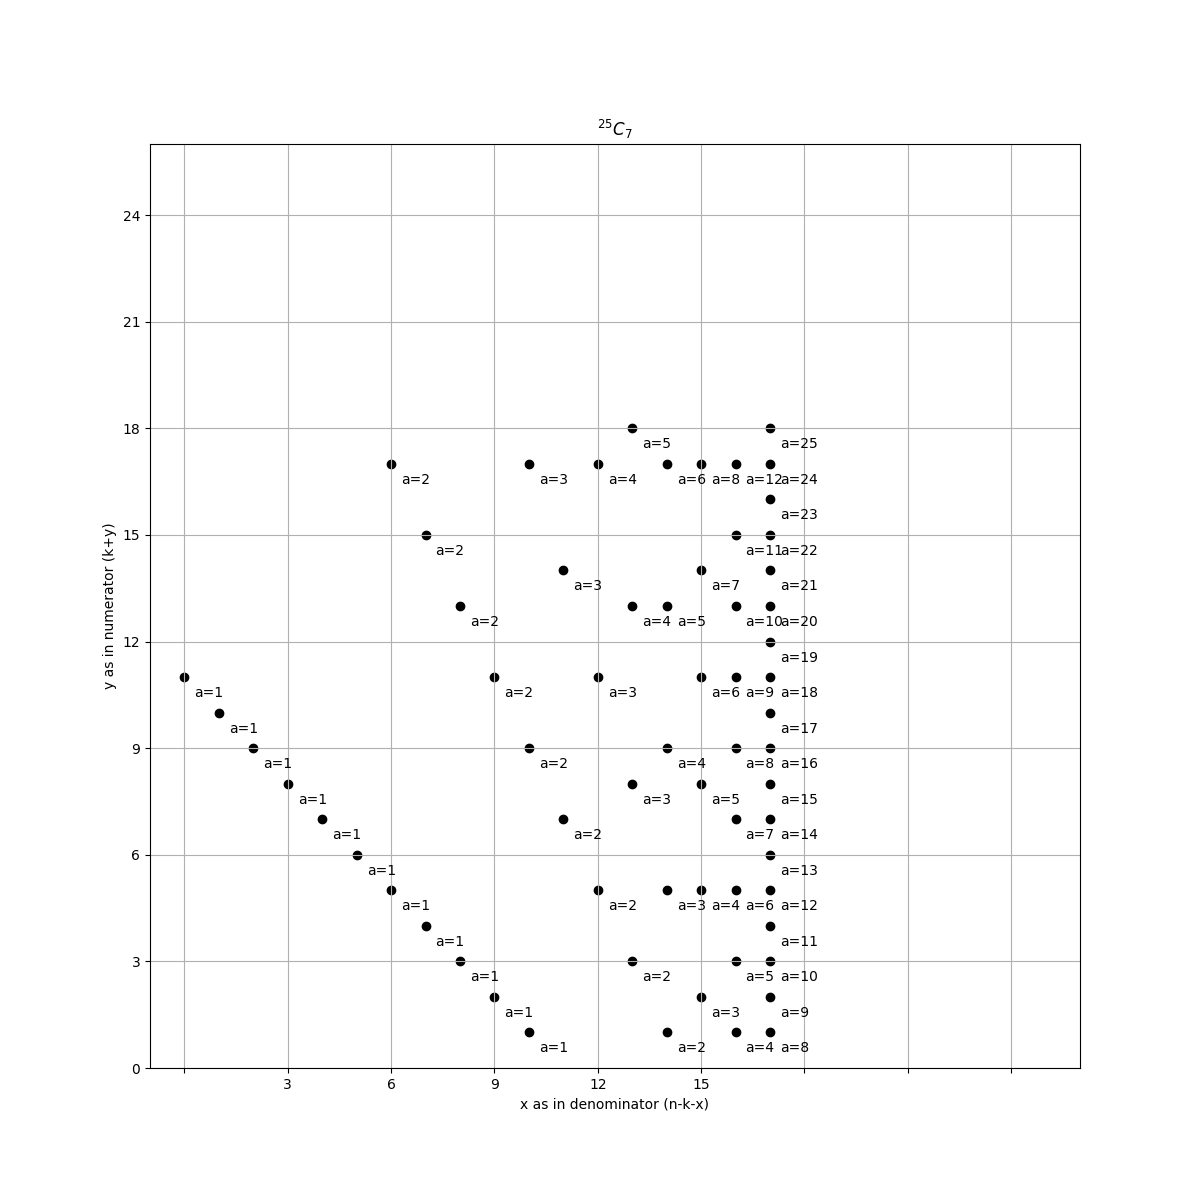
\includegraphics[width=\linewidth]{25_7_alone.png}
	\caption{Distribution of $x,y \text{ and } a$ in the graph of $\Combination{25}{7}$}
	\label{25_C_7_example}
\end{figure}
\begin{figure}[ph!]
	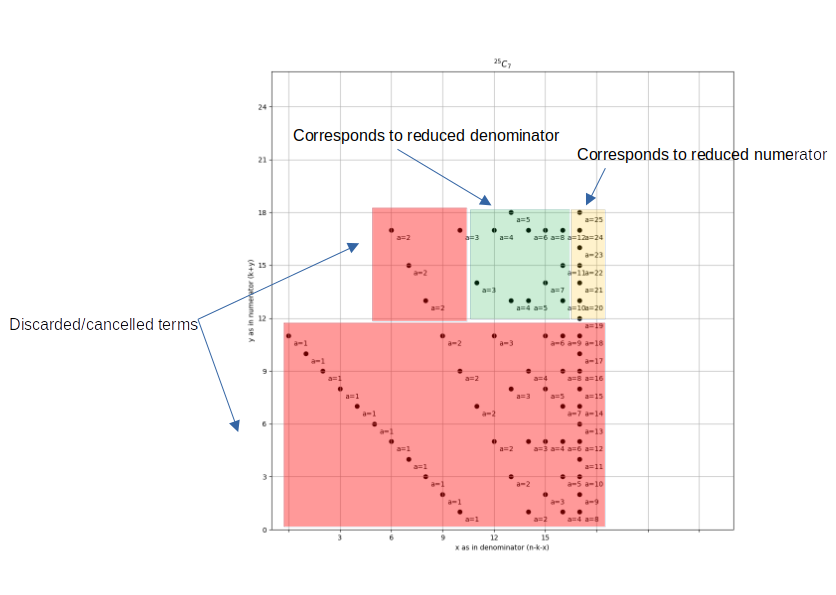
\includegraphics[width=\linewidth]{CalculationOfCombination.png}
	\caption{Showing set of numerator and denominator terms $\Combination{25}{7}$}
	\label{CalculationOfCombination}
\end{figure}
\begin{figure}[ph!]
	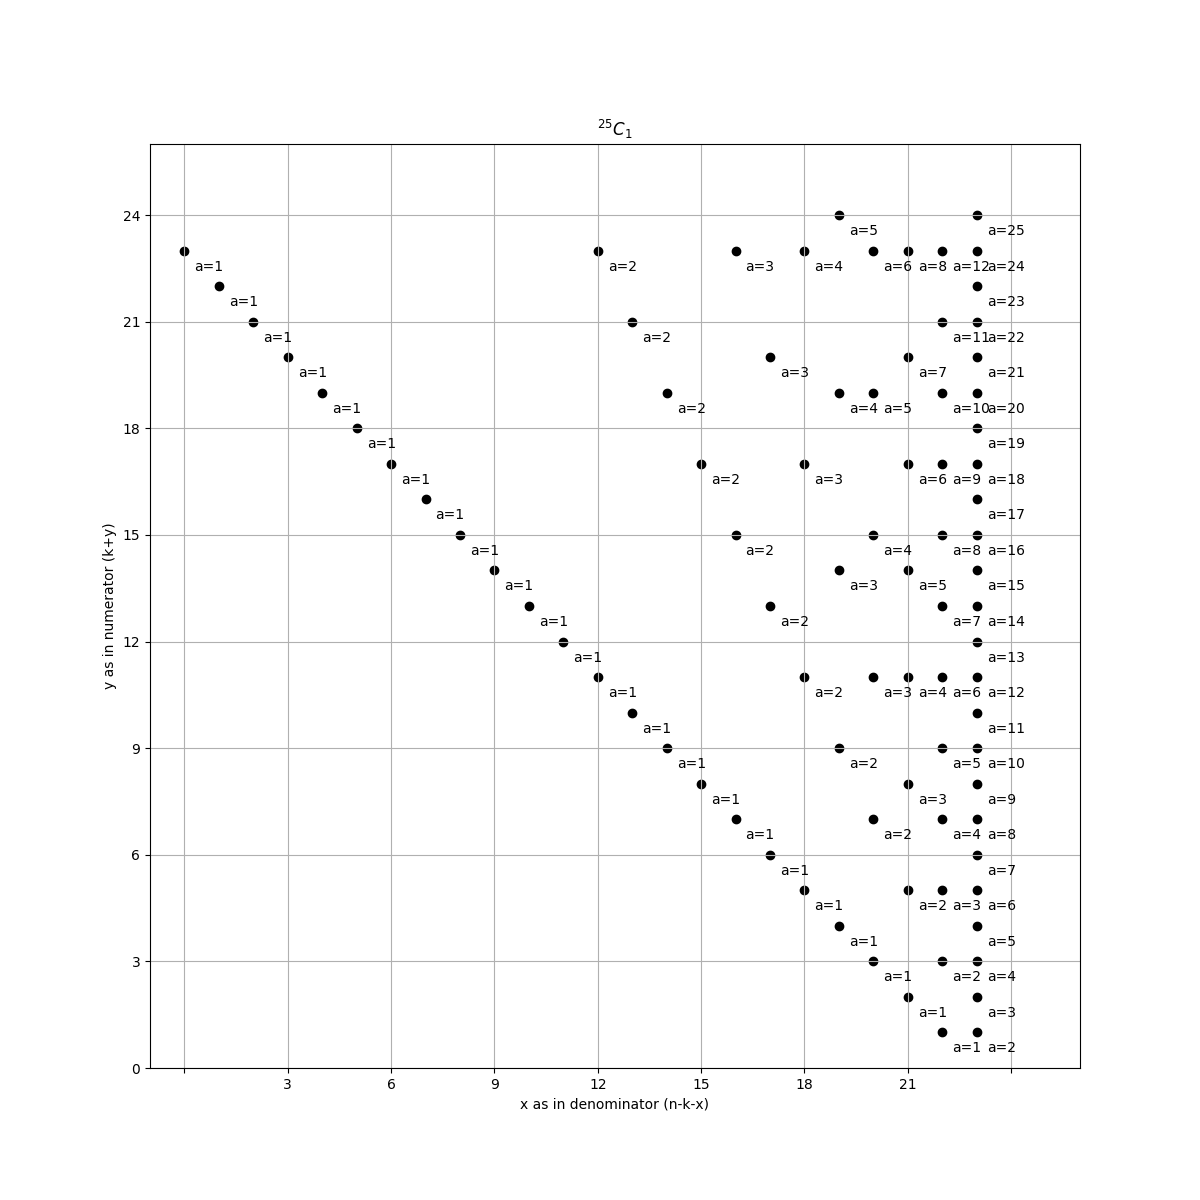
\includegraphics[width=\linewidth]{25_1_alone.png}
	\caption{Distribution of $x,y \text{ and } a$ in the graph of $\Combination{25}{1}$}
	\label{25_C_1_example}
\end{figure}
\end{document}